\section{Research on Methodologies}
\subsection{Agile}
As software engineers from TU Delft, we've been taught to use Agile methods, specifically, the Scrum method, wherein engineers create a feedback loop based on what has been done, and what needs to be done, having regular meetings where progress is reviewed, and brief planning is done for the near future. In most Agile methods, immediate productivity and risk reduction are put to the forefront, which, specifically in the Scrum method takes, place through constant meetings with the client and with the teams, to assess difficulties, changes in requirements, and specifications, all in the name of reducing risks with regards to the final product \cite{agilesource}. Following the release of the \href{https://agilemanifesto.org/}{Manifesto for Agile Software Development}, these methods have become highly popular, as they stray away from the previously bloated, long-winded development models, such as the Waterfall \cite{manifest}. Agile methods are practical, as they focus on simplicity, constantly working software, and welcome changes in the specifications or requirements \cite{beck2001agile}. This is where Agile methods strive: simply producing results in environments where the engineers just have to make a working system, however, we find that there are some limitations to Agile and its simple, incremental style. The lightweight framework, although very efficient for simply writing code, has little in the way of documentation, prototyping, and formal studies, making the steps following production (operating, maintenance, and deployment) potentially more difficult than they have to be. As our client is an extremely large company, and they've explicitly mentioned that they hope to continue maintaining, modifying, and deploying our system after we have finished, we find the steps after \textbf{our} production life-cycle to be extremely important. For this reason, among others, we explored alternatives to Agile \cite{relation}.

\subsection{Waterfall}
The Waterfall model is a process method that, recently, has been less popular due to the rise of practicality-focused Agile methods, however, its apparent decline in popularity does not mean it is necessarily inferior. The Waterfall model belongs to a class of process models called Document-driven models, which, contrary to Agile models, have clearly defined stages, which are demarcated by detailed documents \cite{spiralmode;}. Although some may not see the value in spending time creating documents for each stage, having documentation to reference later on, whether it be for the same team, new members, or different team picking up where another left off, documentation, especially depicting choices in design are an invaluable resource, which is often not given explicit time in Agile methods. Furthermore, the Waterfall method is linear, assuming that each steps occur one after the other and that teams often shouldn't have to go back, unless something goes wrong. Given that we intend to make a robust system to hand off to AWS after the completion of this project, detailed documents after each are extremely useful. This methodology also has extremely clear milestones, which, although there will not be a working system at each step, the client will have some sort of idea of how the project is going with the documents. Despite this, the Waterfall model certainly isn't perfect. Given the robust and sequential nature of the model, it is rather inflexible, as changes to the requirements, according to the model, are not able to be accounted for without going back and editing every after the first one that was changed. Furthermore, since prototyping and experimentation don't occur until later, errors may be detected rather late, which, given the short-lived nature of this project, we certainly cannot afford \cite{comparitvestudy}.

\begin{figure}[H]
\centering
\begin{subfigure}{0.5\textwidth}
  \centering
  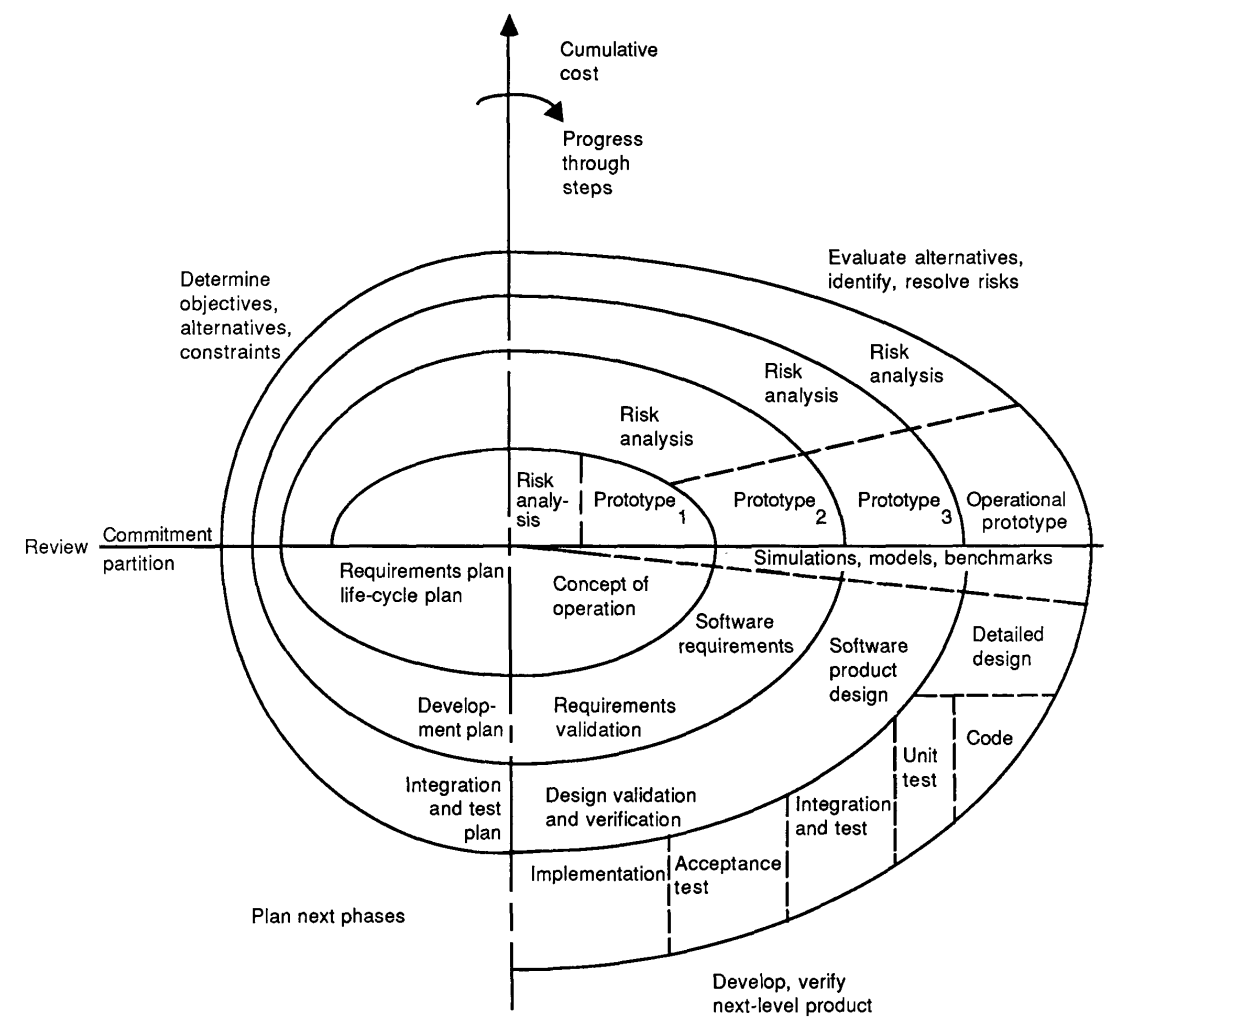
\includegraphics[width=.4\linewidth]{images/Spiral Model.png}
  \caption{Spiral model \cite{spiralmode;}}
  \label{fig:sub1}
\end{subfigure}%
\begin{subfigure}{0.5\textwidth}
  \centering
  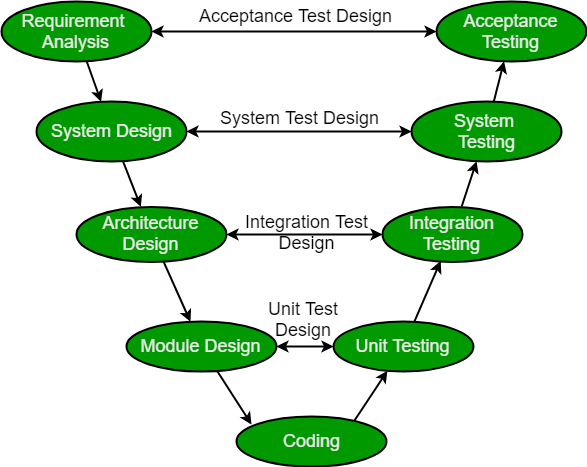
\includegraphics[width=.4\linewidth]{images/vee.png}
  \caption{Vee model \cite{geeksforgeeks_2023}}
  \label{fig:sub2}
\end{subfigure}
\caption{The Spiral and Vee models side by side}
\label{fig:test}
\end{figure}

\subsection{Waterfall Derivatives: Spiral and Vee}
From the Waterfall model, came many improvements, the two most notable that we have considered are the Vee model and the Spiral model \cite{spiralmode;} \cite{geeksforgeeks_2023}. The spiral model builds on top of the Waterfall by creating an iterative approach in the planning phase, wherein each phase risks are assessed and analyzed, a prototype is created, and more information is contextualized for the next phase, making the successive iterations more detailed, yet time-consuming. This model does not appear to have much in the way of dictating how the implementation steps are to be carried out, as by the time actual implementation is to occur, the documents depicting the software should have been already written, with only the fine-grained details being necessary for the final spiral. Alternatively, for our purpose, the prototypes could be adapted for high-level iterations toward the final working product. The Vee Model builds on top of the Waterfall model by being linear, however, adds explicit many explicit verification and validation steps. The model suggests that software engineering is at the highest level, verifying the requirements at each step, and then after code completion, through testing, work its way back up, going through steps of unit testing, integration testing, etc. \cite{geeksforgeeks_2023}. These validation steps work in tandem with the verification steps in terms of abstraction, ensuring that they meet and align with each other, oftentimes being done in parallel. With all this information in mind, it is important to remember the purpose of a process model: "Thus, a process model addresses the following software project questions: (1) What shall we do next? (2) How long shall we continue to do it. \cite{spiralmode;}"
